%%%%%%%%%%%%%%%%%%%%%%%%%%%%%%%%%%%%%%%%%%%%%%%%%%%%
\documentclass[fleqn,10pt,twocolumn]{AROB}

\title{Preparation of Papers in a Two-Column Format for\\
       AROB 2026 with \LaTeX }

\author{Taro Mure${}^{1\dagger}$ and Hanako Gun${}^{2}$}
% The dagger symbol indicates the presenter.
\speaker{Taro Mure}

\affils{${}^{1}$Department of Xxx, University of Xxxx, Okinawa, Japan\\
(Tel: +81-2-000-0000; E-mail: taro@xxx.ac.jp)\\
${}^{2}$Department of Yyy, Yyyy University, Okinawa, Japan\\
(Tel: +81-3-000-0000; E-mail: hanako@yyyy.ac.jp)\\
}
\abstract{%
This template provides a sample format of final manuscripts
for AROB 2026.  It also provides instructions to
authors for completing the final manuscripts which will be
included in the conference Proceedings.
This template is available for abstracts, short and full papers. }

\keywords{%
Selected keywords relevant to the subject.
}

\begin{document}

\maketitle

%-----------------------------------------------------------------------

\section{Introduction}

Each paper must consist of two parts. The first part contains the paper title, authors�f names, abstract, and keywords. The second part is the main body of the paper.

\section{Page size and format}

The manuscript must be in A4-sized single-spaced double-column format.
%
We offer two options for submission: either a full paper or a short paper.
%
Please note that the short paper option is only available to OS speakers who get a permission from the corresponding OS organizer. If you get the permission, please inform the program chair, Prof. Fumitoshi Matsuno (fumitoshi.matsuno[at]oit.ac.jp*) and the AROB secretariat (arobsecr[at]isarob.org) by 1 December.
%
The only difference between the formats of these options is the number of maximum pages.
%
Full papers should have a minimum length of 4 pages and a maximum length of 6 pages, and should report on new unpublished work. Short papers are limited to a 2-page length and can report on previously published work, but are expected to provide new insights. Also, an abstract is not required for short papers. Both types of papers can have figures and tables within the corresponding page limits.
%
See the conference website for more details.

%\begin{table}
\begin{center}
\begin{tabular}{lc}
    Left margin  &  15mm \\
    Right margin &  15mm \\
    Top margin   &  30mm \\
    Bottom margin&  25mm \\
    Column width &  85mm \\
\end{tabular}
\end{center}
%\end{table}

Submitted papers MUST BE in Portable Document Format (PDF).  NO OTHER
FORMATS WILL BE ACCEPTED.

\section{Fonts and style}

\subsection{First part}

The first part includes the paper title, authors' name, abstract, and
keywords, all of them in Times Roman or similar font.  The font
size of the title, authors' name, affiliation, abstract, and keywords
are bold 12pt, 11pt, 10pt, 10pt, and 10pt, respectively.

\subsection{Paper body}

The second part consisting of the body of the paper must be edited in
double column format, with each column 80mm width and separated by
10mm.  The top-level heading, usually called section, numbered in
Arabic numerals, shall appear centered on the column with Times Roman
capital bold 11pt.  The numbered level-two heading starts from the
left in Times Roman bold 10pt font.  The main text uses Times Roman
10pt font with single spacing.  The first line of a new paragraph is
indented by 4mm.

\section{Figures, tables, and equations}

\subsection{Figures and tables}

Place figures and tables at the top or bottom of columns.
Avoid placing them before their first mention in the text.
Large figures and tables may span across both columns.
Scanned images (e.g., line art, photos) can be used if the output
resolution is at least 600dpi.

\begin{table}[b]
\caption{Caption should be placed above the table.}
\begin{center}
\begin{tabular}{|c|c|c|c|}\hline
    &   A   &   B   &   C \\\hline
(1) & 150\% & 16.3\% & 18.2\% \\\hline
\end{tabular}
\end{center}
\end{table}


\begin{figure}[b]
\begin{center}
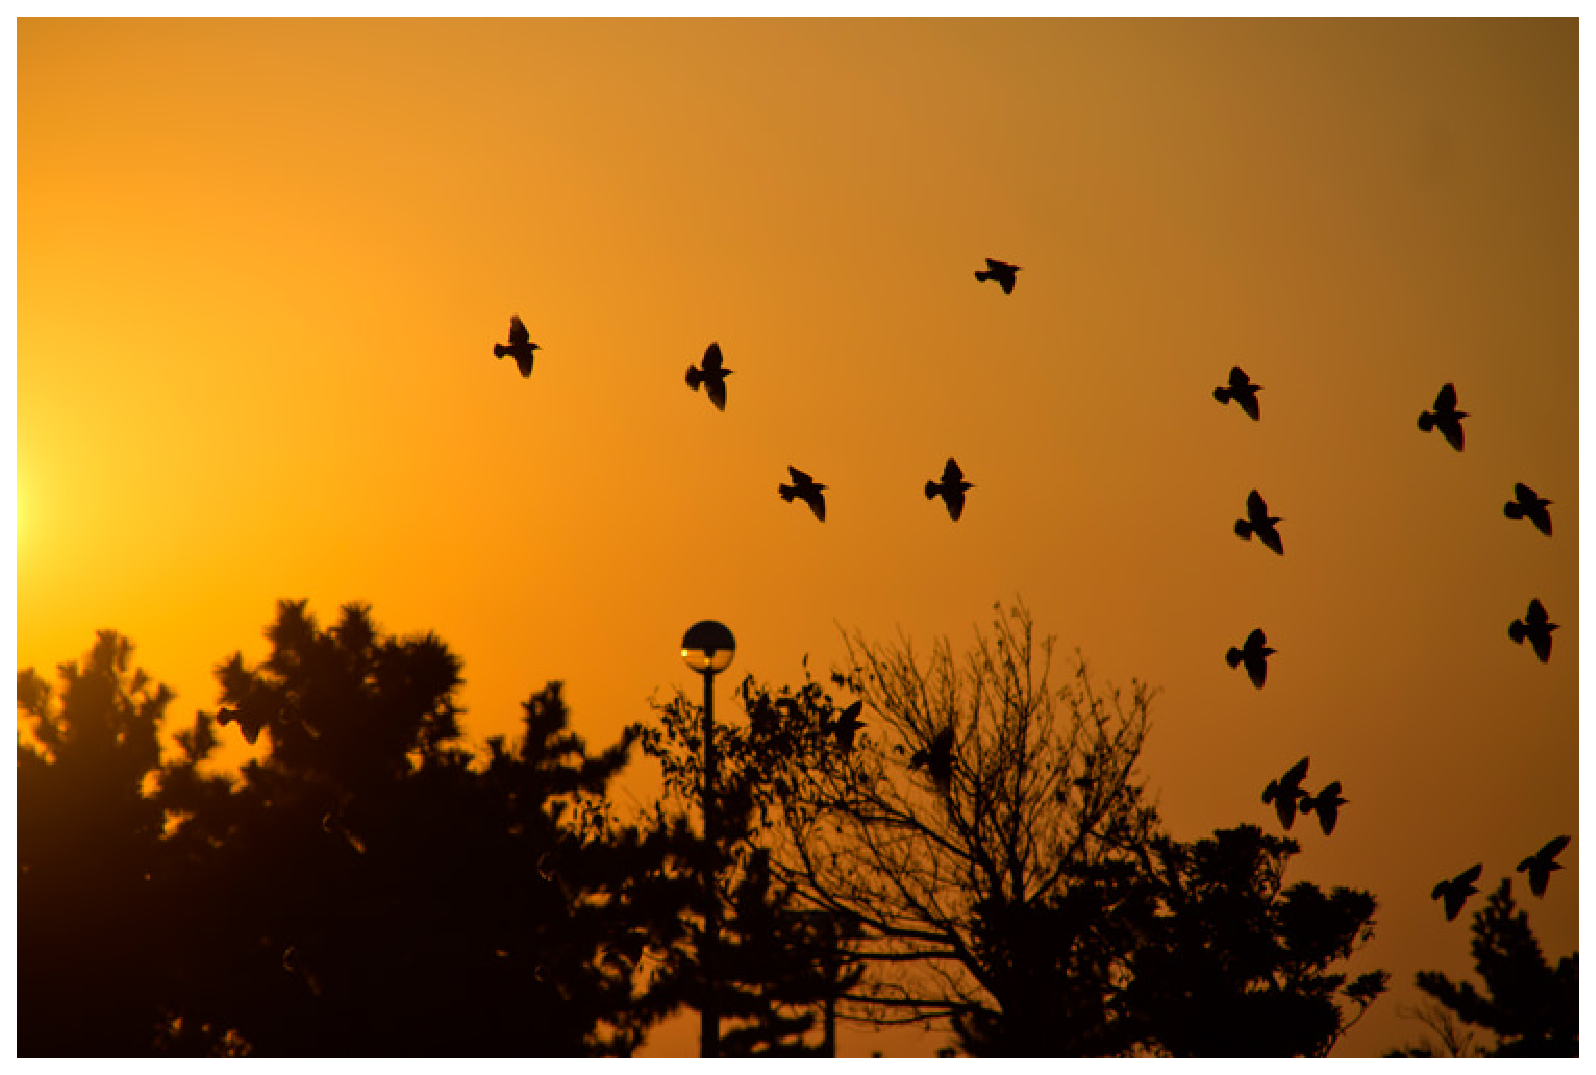
\includegraphics[width=8cm]{AROB_fig.eps}
\caption{\label{test} Caption should be placed below the figure.}
\end{center}
\end{figure}

Figure captions should be below the figures; table captions should
be above the tables.  They should be referred to in the text, for
example, Fig. \ref{test}, or Figs. 1 to 3.

\subsection{Equations}

Equation numbers should be Arabic numerals enclosed in parentheses on
the right-hand margin.  They should be cited in the text as, for
example, Eq. (\ref{eq:ss}), or Eqs. (1) to (3).  Equations start
from the left of the column.  Punctuate equations with commas or
periods when they are part of a sentence.  For example,

\begin{eqnarray}
\begin{array}{rcl}
\dot{x}&=&Ax+Bu,\\
y&=&Cx+Du,
\end{array}
\label{eq:ss}
\end{eqnarray}
where $x$ is the state vector.

\subsection{References}

References should appear in a separate bibliography at the end of the
paper, with items referred to with numerals in square brackets
\cite{ref1,ref3,ref4,ref5}.  Times Roman 10pt is used for references.

\section{PAGE NUMBERS}

Do not put page numbers in the manuscript PDF.

%%%%%%%%%%%%%%%%% BIBLIOGRAPHY IN THE LaTeX file !!!!! %%%%%%%%%%%%%%%%%%%%%%
\begin{thebibliography}{9}
\bibitem{ref1}
AROB 2026 Website,\\ ``https://isarob.org/symposium/''

\bibitem{ref2}
T. Mure, ``XXX Control of Nonlinear Systems'',
{\it International Journal of YYY}, Vol. 99, No. 99, pp. 123--456, 2012.

\bibitem{ref3}
H. Gun, {\it ZZZ Handbook}, SICE, Tokyo, 2012.

\bibitem{ref4}
T. Mure, ``Measurement Method using ABC Sensor'', {\it Transaction of EFG}, 
Vol. 00, No. 1, pp. 1--9, 2011.

\bibitem{ref5}
H. Gun, ``SSS Intelligent Systems'', {\it International Journal of VVV}, 
Vol. 12, No. 5, pp. 500--600, 2011.

\end{thebibliography}

\end{document}
